\documentclass[11pt,a4paper]{article}
\usepackage[utf8]{inputenc}
\usepackage[T1]{fontenc}
\usepackage[margin=2.5cm]{geometry}
\usepackage{amsmath,amssymb}
\usepackage{booktabs}
\usepackage{longtable}
\usepackage{graphicx}
\usepackage{xcolor}
\usepackage{listings}
\usepackage{hyperref}
\usepackage{caption}
\usepackage{enumitem}
\emergencystretch=2em

\lstset{language=C++, basicstyle=\ttfamily\footnotesize, keywordstyle=\color{blue!70!black},
  commentstyle=\color{green!45!black}, stringstyle=\color{red!60!black},
  showstringspaces=false, breaklines=true, frame=single, columns=fullflexible,
  xleftmargin=4pt, framexleftmargin=4pt}

\title{Methods and Models for Combinatorial Optimization\\[4pt]
  \large Lab exercises: an exact method and a tabu search for the drilling sequence problem}
\author{Riccardo Fabbian, 2140711\\ University of Padova}
\date{September 2026}

\begin{document}
\maketitle

\begin{abstract}
A drilling machine must make $n$ holes on a board and come back to the first hole so that the
next board can be processed. Since the drilling time is the same for every hole, the sequence
that minimises the total processing time is the one that minimises the travelling time of the
drill, i.e.\ a minimum-cost Hamiltonian cycle on the holes: a Travelling Salesman Problem.
This report describes two ways of solving it. Part~I implements the flow-based integer linear
programming model proposed in the exercise text with the CPLEX Callable Library and measures,
on a benchmark of 50 instances with 10 to 100 holes, up to which size the model can be solved
to proven optimality in 0.1, 1, 10 and 60 seconds. Part~II implements a tabu search on the
2-opt neighbourhood, calibrates its parameters on a separate set of instances and compares it
with the exact method at equal time budgets. The exact method proves optimality for boards of
10, 20, 40 and 60 holes within the four budgets; the tabu search returns the optimum of every
instance up to 50 holes in a tenth of a second and up to 90 holes in one second, and stays
within half a percent of the best known value at 100 holes.
\end{abstract}
\newpage
\tableofcontents
\vspace{2em}

%=====================================================================
\section{Introduction}
%=====================================================================
The exercise asks to solve the same combinatorial optimization problem with two different
tools: a mathematical programming model handed to a general-purpose solver, which returns a
provably optimal solution but may take a very long time, and a metaheuristic, which returns a
good solution quickly but without any guarantee. The interest of the exercise lies in seeing
where each of the two stops being useful, on the same instances and with the same time.

The report is organised as follows. Section~\ref{sec:problem} describes the problem, its
formulation as a TSP and the instances used in the experiments. Section~\ref{sec:assignment1}
presents the mathematical model, how it was implemented with the CPLEX API and the results of
the exact method, with the answer to the question of the exercise (up to which size the model
can be solved in a given time). Section~\ref{sec:assignment2} presents the tabu search: its
components, the design decisions that were taken and why, the calibration of its parameters
and the results, compared with those of Part~I. Section~\ref{sec:env} documents the machines
and the way times were measured, and Section~\ref{sec:concl} draws the conclusions.

\subsection{Project structure}
The code is written in C++ (standard C++11, so that it compiles with the compiler of the
laboratory machines) and organised as follows.
{\small\begin{verbatim}
project/
  Makefile            builds tsp_cplex (Part I) and tsp_tabu (Part II)
  README.md           options of the programs and how to reproduce the experiments
  common/
    instance.h        instance reader, cost matrix, tour utilities
    timer.h           wall-clock stopwatch
  assignment_1/
    main.cpp          command line, output of one CSV line per run
    tsp_model.h/.cpp  class TSPModel: builds and solves the flow model with CPLEX
    cpxmacro.h        CPLEX helper macros of the laboratory
  assignment_2/
    main.cpp          command line, output of one CSV line per run
    tabu_search.*     class TabuSearch
  instances/          50 benchmark instances, 8 calibration instances
  scripts/            instance generator, campaign scripts, analysis
  results/            CSV output of every run, results/tables/ (tables of this report)
  report/             this report
\end{verbatim}}
Both programs take an instance file as argument, solve it and print a single line of
comma-separated values (status, objective value, times, \ldots), so that a campaign over many
instances is a shell loop whose output is directly a CSV file; the tables and figures of this
report are produced from those files by \texttt{scripts/analyze.py}. Building and running are
described in Section~\ref{sec:build}.

%=====================================================================
\section{The problem and the instances}\label{sec:problem}
%=====================================================================
\subsection{From the drilling machine to the TSP}
A company produces boards with holes used to build electric panels. A board is positioned on
a machine, a drill moves over it, stops at the position of each hole and drills; once the
board is finished a new one is positioned and the process starts again, so the drill must
come back to the first hole. The time needed to make a hole is the same for all the holes.
The company wants the sequence of holes that minimises the total time needed to drill a
board.

The total time is the sum of two parts: the drilling time, $n$ times a constant, and the
moving time between consecutive holes. The first part is the same for every sequence, so
only the second one has to be minimised. This is the situation modelled by the Travelling
Salesman Problem. Every hole is a node of a complete directed graph $G=(N,A)$; every move of
the drill from hole $i$ to hole $j$ is an arc $(i,j)\in A$ with a cost $c_{ij}$ equal to the
moving time. A drilling sequence that makes every hole once and comes back to the start is a
cycle of $G$ visiting every node exactly once, a Hamiltonian cycle, and the best sequence is
the Hamiltonian cycle of minimum total cost.

\paragraph{The cost of a move.}
I assume that the drill head moves in a straight line at constant speed, so that the moving
time is proportional to the Euclidean distance between the two holes; the distance itself is
used as cost,
\[
  c_{ij} = \sqrt{(x_i-x_j)^2+(y_i-y_j)^2},
\]
with $(x_i,y_i)$ the coordinates of hole $i$. Any other machine could be modelled by changing
this one function: a head that moves one axis at a time would have Manhattan costs
$|x_i-x_j|+|y_i-y_j|$, a head whose axes move simultaneously at the same speed would have
$\max(|x_i-x_j|,|y_i-y_j|)$. Two properties of the Euclidean cost are used later. It is
\emph{symmetric}, $c_{ij}=c_{ji}$, which allows the incremental evaluation of the 2-opt move in
Part~II. It is a \emph{real number}: costs are kept as double-precision values and are never
rounded, so the objective value of the model is a real number too.

\subsection{Instance generator}\label{sec:gen}
An instance is simply a list of hole positions. I generate them on a $100\times100$~mm board,
a plausible size for an electric panel. The generator (\texttt{scripts/gen\_instances.py})
draws the coordinates uniformly at random on the board, with one constraint: two holes must be
at least 1~mm apart, because a drill cannot make two overlapping holes. A candidate point that
violates the constraint is discarded and drawn again. The instance file contains the number of
holes on the first line and then one line ``$x\ y$'' per hole, in millimetres with two
decimals:
\begin{verbatim}
10
11.91 50.25
51.18 86.00
10.26 22.33
...
\end{verbatim}
Costs are not stored in the file: they are computed from the coordinates when the file is read
(\texttt{Instance::computeCosts} in \texttt{common/instance.h}), which keeps the files small
and makes the cost function a single, replaceable piece of code.

The generator uses a fixed random seed, so the benchmark can be regenerated identically and
every result of this report can be reproduced. It produces two sets of instances.
\begin{description}[style=nextline]
  \item[Benchmark set (seed 2026).] Sizes $n\in\{10,20,30,\dots,100\}$, five instances per
    size, 50 instances in total, named \texttt{tsp\_n<size>\_<k>.dat}. All the results of
    Parts~I and~II are measured on these instances. Five instances per size are needed
    because, as Section~\ref{sec:p1results} shows, the time the exact method needs varies by
    an order of magnitude between instances of the same size: a single instance per size would
    give a very noisy answer to the question of the exercise.
  \item[Calibration set (seed 7).] Sizes $n\in\{30,50,70,100\}$, two instances per size,
    named \texttt{calib\_n<size>\_<k>.dat}. These are used only to calibrate the parameters of
    the tabu search (Section~\ref{sec:calib}). Keeping the calibration instances separate from
    the benchmark is the same discipline as keeping a training set separate from a test set:
    parameters tuned on the very instances used to report results would give an
    optimistic picture of the algorithm.
\end{description}
Figure~\ref{fig:tour} shows one of the benchmark instances together with its optimal tour.

%=====================================================================
\section{Part I: exact method with CPLEX}\label{sec:assignment1}
%=====================================================================
\subsection{Mathematical model}\label{sec:model}
Several integer linear programming formulations of the TSP exist. The classical one, with
the subtour elimination constraints of Dantzig, Fulkerson and Johnson, has an exponential
number of constraints (one for every subset of nodes) and cannot be handed to the solver in
one piece: it needs a procedure that generates the violated constraints on demand. The
exercise asks for a \emph{compact} formulation, one with a polynomial number of variables and
constraints, and suggests the single-commodity flow formulation of Gavish and Graves, which
I implement.

The idea is the following. Choose an arbitrary hole as starting node, call it node~0, and
imagine that it sends $n-1$ units of a fictitious commodity into the network. Every other node
must receive exactly one unit and forward the rest; the commodity can travel only on the arcs
used by the drill. As shown below, these two requirements together force the used arcs to
form a single cycle through all the nodes.

\paragraph{Sets and parameters.}
$N$ is the set of holes and $A$ the set of arcs $(i,j)$, $i\neq j$; $c_{ij}$ is the cost of
arc $(i,j)$; $0\in N$ is the starting hole.

\paragraph{Decision variables.}
$y_{ij}\in\{0,1\}$ is 1 if the drill moves directly from hole $i$ to hole $j$, 0 otherwise;
$x_{ij}\ge0$ is the amount of flow shipped on arc $(i,j)$.

\paragraph{Model.}
\begin{align}
  \min\; & \sum_{(i,j)\in A} c_{ij}\, y_{ij} \label{eq:obj}\\
  \text{s.t.}\;
  & \sum_{i:(i,k)\in A} x_{ik} - \sum_{j:(k,j)\in A,\, j\neq 0} x_{kj} = 1 & \forall k\in N\setminus\{0\} \label{eq:flow}\\
  & \sum_{j:(i,j)\in A} y_{ij} = 1 & \forall i\in N \label{eq:out}\\
  & \sum_{i:(i,j)\in A} y_{ij} = 1 & \forall j\in N \label{eq:in}\\
  & x_{ij} \le (n-1)\, y_{ij} & \forall (i,j)\in A,\ j\neq 0 \label{eq:link}\\
  & x_{ij} \in \mathbb{R}_+ \quad \forall (i,j)\in A,\ j\neq 0, \qquad y_{ij}\in\{0,1\} \quad \forall (i,j)\in A. \nonumber
\end{align}

The objective \eqref{eq:obj} is the total cost of the arcs travelled by the drill. Constraints
\eqref{eq:out} and \eqref{eq:in} are the \emph{assignment} constraints: exactly one arc leaves
and exactly one arc enters every hole. Constraint \eqref{eq:flow} is the \emph{flow
conservation} at node $k$: what enters $k$ minus what leaves $k$ is one unit, the unit that
$k$ keeps. Constraint \eqref{eq:link} \emph{links} the two families of variables: if the arc is
not used ($y_{ij}=0$) no flow can travel on it; if it is used, at most $n-1$ units can, which
is all the flow that exists. This is a ``big-M'' constraint of the kind used in the fixed-cost
models seen in the course, with $M=n-1$ being the smallest valid value.

\paragraph{Why the model excludes subtours.}
The assignment constraints alone are satisfied by any set of disjoint cycles covering all
the nodes, not only by Hamiltonian cycles. Consider for example four holes and the two cycles
$0\to1\to0$ and $2\to3\to2$, i.e.\ $y_{01}=y_{10}=y_{23}=y_{32}=1$ and all other $y$ equal to
0: every node has one arc in and one arc out. Now look at the flow. By \eqref{eq:link} the
flow can be positive only on the four used arcs, so the conservation constraints of nodes 2
and 3 read $x_{32}-x_{23}=1$ and $x_{23}-x_{32}=1$; adding them gives $0=2$, which is
impossible. The same argument applies to any cycle $S$ that does not contain node~0: no
used arc enters $S$ from outside, so no flow can reach it, yet each of its $|S|$ nodes should
keep one unit; summing \eqref{eq:flow} over $S$ gives $0=|S|$. Therefore every node must be
reachable from node~0 along used arcs, and with the assignment constraints this means that
the used arcs form a single cycle through all the nodes. On the valid tour $0\to1\to2\to3\to0$,
for instance, the flow is $x_{01}=3$, $x_{12}=2$, $x_{23}=1$: it decreases by one unit at
every hole, like a van that delivers one parcel per stop.

\paragraph{Two simplifications.}
The original model also contains the constraint $\sum_j x_{0j}=n-1$, which fixes the amount
of flow sent by node~0. As remarked in the exercise text it is redundant: the $n-1$
constraints \eqref{eq:flow} absorb $n-1$ units, which can only come from node~0, and sending
more than that is never needed. Moreover, no flow needs to go back to node~0, so the variables
$x_{i0}$ are removed from the model; this is why the second sum of \eqref{eq:flow} and the
linking constraints \eqref{eq:link} exclude $j=0$.

\paragraph{Size of the model.}
There are $(n-1)^2$ flow variables (arcs $(i,j)$ with $j\neq0$), $n(n-1)$ binary variables,
$n-1$ flow constraints, $2n$ assignment constraints and $(n-1)^2$ linking constraints. At
$n=100$ the model has $19\,701$ variables and $10\,100$ constraints; at $n=10$, $171$ and
$110$. The model is compact, as required, but both the number of variables and the number of
constraints grow with $n^2$.

\paragraph{A remark on the strength of the model.}
The solver works by solving the linear relaxation of the model (the same model with
$y_{ij}\in[0,1]$) at every node of a branch-and-bound tree, and the relaxation is a good
guide only if its optimal value is close to the integer optimum. In the flow model the linear
relaxation is weak, and the cause is constraint \eqref{eq:link}: a fractional solution can ship
one unit of flow on an arc with $y_{ij}=1/(n-1)$, paying only a $(n-1)$-th of the arc cost.
The larger the instance, the smaller this fraction and the weaker the bound. This is a
property of the formulation, not of the solver, and it is the reason why, as the results will show, the
exact method slows down so sharply with $n$.

\subsection{Implementation with the CPLEX Callable Library}\label{sec:impl1}
The model is implemented in the class \texttt{TSPModel} (\texttt{assignment\_1/tsp\_model.h},
\texttt{tsp\_model.cpp}) using the C API of CPLEX, with the \texttt{cpxmacro.h} header of the
laboratory. The header provides the macros \texttt{DECL\_ENV} and \texttt{DECL\_PROB}, which
create the CPLEX environment and an empty problem, and \texttt{CHECKED\_CPX\_CALL}, which
calls a CPLEX function, checks its return status and, if it is not zero, throws a C++
exception carrying the CPLEX error message. Every call to the library goes through this
macro, so an error in the construction of the model cannot pass unnoticed. The constructor
creates the environment and the problem and sets the objective sense to minimisation; the
destructor frees them.

\paragraph{Variable indices.}
CPLEX has no notion of ``the variable $y_{ij}$'': it identifies a variable by its position in
the column vector of the problem, an integer assigned when the variable is created. To write
the constraints I therefore need a map from the pair $(i,j)$ to the column position. I use
two $n\times n$ integer matrices, \texttt{xIdx\_} and \texttt{yIdx\_}, initialised to $-1$: the
entry $[i][j]$ holds the column of $x_{ij}$ or $y_{ij}$, and stays $-1$ for the variables
that do not exist ($i=j$ for both families, and $j=0$ for $x$, since the $x_{i0}$ were
removed from the model). The look-up costs $O(1)$ and the two matrices cost $O(n^2)$ memory,
the same order as the cost matrix, so nothing is lost with respect to a hash map or an
arithmetic formula, and the value $-1$ makes any use of a non-existing variable immediately
visible.

\paragraph{Creating the variables.}
Variables are created with one call of \texttt{CPXnewcols} per family, first the $x$ then the
$y$. For each family the code fills five parallel vectors, one entry per variable: objective
coefficient, lower bound, upper bound, type and name. For $x_{ij}$ the coefficient is 0 (flow
has no cost), the bounds are $[0,n-1]$ and the type is \texttt{'C'} (continuous); for $y_{ij}$
the coefficient is $c_{ij}$, the bounds are $[0,1]$ and the type is \texttt{'B'} (binary). While
the vectors are filled, the column position of each variable is recorded in the index matrix:
\begin{lstlisting}
int pos = CPXgetnumcols(env_, lp_);          // columns created so far
for (int i = 0; i < n_; ++i)
    for (int j = 0; j < n_; ++j) {
        if (i == j) continue;
        yIdx_[i][j] = pos++;                    // remember the column of y_ij
        obj.push_back(inst_.cost[i][j]);
        lb.push_back(0.0);  ub.push_back(1.0);  type.push_back('B');
        std::snprintf(name, sizeof name, "y_%d_%d", i, j);
        names.push_back(name);
    }
CHECKED_CPX_CALL(CPXnewcols, env_, lp_, (int)obj.size(), &obj[0], &lb[0], &ub[0],
                 &type[0], &cnames[0]);
\end{lstlisting}
Creating all the variables of a family in one call, instead of one call per variable, is
what the laboratory recommends: CPLEX allocates the columns once instead of growing its
internal arrays $n^2$ times. The names are only used when the model is inspected (for example
with \texttt{CPXwriteprob}); they cost nothing during the solution.

\paragraph{Creating the constraints.}
Constraints are created with one call of \texttt{CPXaddrows} per family, in the sparse row
format used by CPLEX. A set of rows is described by three arrays: \texttt{rmatind} lists the
column indices of all the non-zero coefficients, row after row; \texttt{rmatval} lists the
corresponding coefficients; \texttt{rmatbeg[r]} is the position in the two arrays where row
$r$ starts. Two further arrays give the right-hand side and the sense of every row
(\texttt{'E'} for $=$, \texttt{'L'} for $\le$, \texttt{'G'} for $\ge$). Only the non-zero
coefficients are stored, which is essential here: a flow conservation row has $2n-3$
non-zeros out of about $2n^2$ variables.

\begin{itemize}
  \item \emph{Flow conservation \eqref{eq:flow}.} $n-1$ rows, one for every $k\neq0$; row
    $k$ contains the $n-1$ variables $x_{ik}$ with coefficient $+1$ and the $n-2$ variables
    $x_{kj}$, $j\neq0$, with coefficient $-1$; right-hand side 1, sense \texttt{'E'}.
  \item \emph{Out-degree \eqref{eq:out} and in-degree \eqref{eq:in}.} $2n$ rows; row $i$
    of the first group contains the $n-1$ variables $y_{ij}$, row $j$ of the second the $n-1$
    variables $y_{ij}$, all with coefficient 1; right-hand side 1, sense \texttt{'E'}.
  \item \emph{Linking \eqref{eq:link}.} $(n-1)^2$ rows, one per arc with $j\neq0$. CPLEX
    requires a constant right-hand side, so the constraint is rewritten as
    $x_{ij}-(n-1)\,y_{ij}\le0$: two non-zeros per row, coefficients $1$ and $-(n-1)$,
    right-hand side 0, sense \texttt{'L'}.
\end{itemize}
The code of the flow conservation family illustrates the pattern; the other families are
built in the same way.
\begin{lstlisting}
for (int k = 1; k < n_; ++k) {
    rmatbeg.push_back((int)rmatind.size());        // row k starts here
    for (int i = 0; i < n_; ++i)
        if (i != k) { rmatind.push_back(xIdx_[i][k]); rmatval.push_back(1.0); }
    for (int j = 1; j < n_; ++j)
        if (j != k) { rmatind.push_back(xIdx_[k][j]); rmatval.push_back(-1.0); }
    rhs.push_back(1.0);
    sense.push_back('E');
}
CHECKED_CPX_CALL(CPXaddrows, env_, lp_, 0, (int)rhs.size(), (int)rmatind.size(), &rhs[0],
                 &sense[0], &rmatbeg[0], &rmatind[0], &rmatval[0], NULL, NULL);
\end{lstlisting}
Building the whole model takes about 0.02~s at $n=100$, three orders of magnitude less than
the solution, so the construction is not a concern for the running times.

\paragraph{Solver parameters.}
Three parameters are set before the call to \texttt{CPXmipopt}.
\begin{itemize}
  \item \texttt{CPXPARAM\_TimeLimit}, the time budget of the run in seconds (0.1, 1, 10 or
    60). When the limit is reached CPLEX stops and returns the best solution found so far
    (the \emph{incumbent}) and the best lower bound it has proved.
  \item \texttt{CPXPARAM\_Threads} $=1$. By default CPLEX uses all the cores of the machine
    and runs its branch-and-bound in an opportunistic parallel mode whose results can differ
    from run to run. With one thread the runs are deterministic, the time budget means the
    same on any machine, and the comparison with the tabu search of Part~II, which is
    single-threaded, is fair.
  \item \texttt{CPXPARAM\_MIP\_Tolerances\_MIPGap} $=10^{-6}$. CPLEX stops the search when the
    relative gap between the incumbent and the best bound falls below this tolerance, and
    reports the incumbent as optimal. The default value is $10^{-4}$: with tour lengths of
    several hundred millimetres this would allow CPLEX to stop with a solution up to about
    0.1~mm longer than the optimum and still call it optimal. Since the results of Part~I are
    the reference against which the tabu search is measured, the tolerance is lowered to
    $10^{-6}$, so that a reported optimum is the optimum up to a negligible rounding.
\end{itemize}

\paragraph{Reading the solution.}
After \texttt{CPXmipopt} the program records the status code (\texttt{CPXgetstat}). A run is
counted as \emph{solved} when the status is \texttt{CPXMIP\_OPTIMAL} or
\texttt{CPXMIP\_OPTIMAL\_TOL} (optimal within the gap tolerance); when the time limit is
reached the status is \texttt{CPXMIP\_TIME\_LIM\_FEAS} if an incumbent exists and
\texttt{CPXMIP\_TIME\_LIM\_INFEAS} otherwise. The program then reads the incumbent value
(\texttt{CPXgetobjval}), the best bound (\texttt{CPXgetbestobjval}), the relative gap
(\texttt{CPXgetmiprelgap}) and the number of branch-and-bound nodes explored
(\texttt{CPXgetnodecnt}). Finally the tour is rebuilt from the values of the variables
(\texttt{CPXgetx}): starting from hole~0, the program repeatedly looks for the $j$ with
$y_{\text{cur},j}>0.5$ and moves there. It then checks that the walk visited every hole
exactly once and came back to hole~0 (so that a subtour would be detected), and that the
length of the tour, recomputed from the cost matrix, equals the objective value returned by
CPLEX. Every run reported in this document passed this check.

\subsection{Computational results}\label{sec:p1results}
Every one of the 50 benchmark instances was solved four times, with a time limit of 0.1, 1,
10 and 60~s. It is important to run the four campaigns separately rather than deducing the
shorter budgets from the 60~s run: CPLEX adapts its strategy to the time it is given, and I
observed that the instances that were solved within the 1~s budget took on average 0.22~s
with that limit and 0.50~s with the 10~s limit. An instance that finishes in 4~s when
the limit is 60~s is therefore not guaranteed to finish when the limit is 10~s, and the only
reliable answer to ``what can be solved in $T$ seconds'' is obtained by running with the limit
$T$.

The full results, instance by instance, are in Table~\ref{tab:p1inst}: for every instance
and budget the table gives the solution time when the instance was solved, and otherwise
the relative gap $(\text{incumbent}-\text{bound})/\text{incumbent}$ reported by CPLEX when it
stopped. Table~\ref{tab:p1} summarises them by size: how many of the five instances were
solved to proven optimality, the average solution time of those, and the average gap of the
others.

\begin{table}[htbp]\centering\small
\caption{Part I, summary by size: instances solved to optimality (out of 5), average solution
time of the solved instances and average gap of the unsolved ones, for every time budget.}
\label{tab:p1}
\resizebox{\textwidth}{!}{\begin{tabular}{rcccccccccccc}
\toprule
& \multicolumn{3}{c}{0.1 s} & \multicolumn{3}{c}{1 s} & \multicolumn{3}{c}{10 s} & \multicolumn{3}{c}{60 s} \\
\cmidrule(lr){2-4} \cmidrule(lr){5-7} \cmidrule(lr){8-10} \cmidrule(lr){11-13}
$n$ & solved & time (s) & gap (\%)& solved & time (s) & gap (\%)& solved & time (s) & gap (\%)& solved & time (s) & gap (\%) \\
\midrule
10 & 5/5 & 0.04 & -- & 5/5 & 0.03 & -- & 5/5 & 0.07 & -- & 5/5 & 0.07 & -- \\
20 & 0/5 & -- & 64.1 & 5/5 & 0.24 & -- & 5/5 & 0.52 & -- & 5/5 & 0.53 & -- \\
30 & 0/5 & -- & 71.4 & 2/5 & 0.30 & 1.6 & 5/5 & 1.85 & -- & 5/5 & 1.85 & -- \\
40 & 0/5 & -- & 77.7 & 2/5 & 0.29 & 17.0 & 5/5 & 2.59 & -- & 5/5 & 2.57 & -- \\
50 & 0/5 & -- & 89.5 & 1/5 & 0.79 & 45.1 & 3/5 & 3.75 & 26.8 & 5/5 & 14.42 & -- \\
60 & 0/5 & -- & 100.0 & 0/5 & -- & 81.4 & 1/5 & 3.51 & 29.5 & 5/5 & 35.34 & -- \\
70 & 0/5 & -- & 100.0 & 0/5 & -- & 83.6 & 1/5 & 4.65 & 17.8 & 4/5 & 28.37 & 47.4 \\
80 & 0/5 & -- & 100.0 & 0/5 & -- & 100.0 & 0/5 & -- & 63.9 & 2/5 & 51.80 & 8.3 \\
90 & 0/5 & -- & 100.0 & 0/5 & -- & 100.0 & 0/5 & -- & 85.5 & 2/5 & 49.86 & 18.3 \\
100 & 0/5 & -- & 100.0 & 0/5 & -- & 100.0 & 0/5 & -- & 87.2 & 0/5 & -- & 6.3 \\
\bottomrule
\end{tabular}
}
\end{table}

\paragraph{Answer to the question of the exercise.}
Taking the strict reading, in which all five instances of a size must be solved to proven
optimality, the flow model solves boards of \textbf{10 holes in 0.1~s, 20 holes in 1~s, 40
holes in 10~s and 60 holes in 60~s}. Taking the loose reading, in which at least one instance
of the size is solved, the limits move to 10, 50, 70 and 90 holes. The difference between the
two readings is a measure of how much the difficulty varies between instances of the same
size: at $n=50$ with 10~s, three instances are solved in 3.7~s on average and two are not
solved at all; at $n=70$ with 60~s, four are solved and one stops with a gap of 47\%. This
variance is intrinsic to the problem (it depends on how well the linear relaxation happens
to describe the particular instance) and is the reason why several instances per size are
necessary.

Every tenfold increase of the budget buys roughly 20 extra holes, and the increments do not
grow with the budget. This is the practical face of an NP-hard problem: the effort grows
exponentially with the size, so a constant factor of time buys a constant increment of size.
Extrapolating the trend, a board of 200 holes would need hours, one of 500 holes would be out
of reach. This is the motivation for Part~II.

\paragraph{What happens inside the solver.}
Some details of Tables~\ref{tab:p1} and~\ref{tab:p1inst} show \emph{how} the difficulty grows.
\begin{itemize}
  \item Up to $n=60$ many instances are closed \emph{at the root node}: 15 of the 38 instances
    solved within 60~s report zero branch-and-bound nodes, which means that the cuts and the
    primal heuristics CPLEX applies to the linear relaxation at the root were enough to find
    the optimum and prove it. Branching becomes systematic from $n=50$, with hundreds of nodes
    per instance, and the solution time grows steeply: 2.6~s at $n=40$, 14~s at $n=50$, 35~s at
    $n=60$ on average, with a maximum of 57~s at $n=70$. Figure~\ref{fig:time} shows the
    solution time of every instance with the 60~s budget: the spread within a size reaches
    an order of magnitude, and the trend of the solved instances is exponential in $n$.
  \item A feasible solution is always found, even with 0.1~s, because CPLEX runs a heuristic
    before starting the search; but for the unsolved instances this solution is of poor
    quality. With 0.1~s the incumbent is 1.6 to 6.7 times longer than the best known tour from
    $n=20$ upwards, and the reported gap is 100\% (CPLEX has not yet computed any useful bound).
    The gap of the unsolved instances shrinks with the budget, but slowly: at $n=100$ it is
    still 6.3\% after 60~s, and on the 12 instances not closed in 60~s the incumbent is on
    average 17\% longer than the best tour found by the tabu search of Part~II.
  \item On the instances it cannot close, CPLEX still provides a valid lower bound. For the 12
    unsolved instances the bound is on average 1.2\% (at most 3.2\%) below the best tour found
    by the tabu search. This is a useful by-product of the exact method: it certifies that
    those heuristic tours are within a few percent of the optimum even though the optimum
    itself is unknown.
\end{itemize}

\begin{figure}[htbp]\centering
  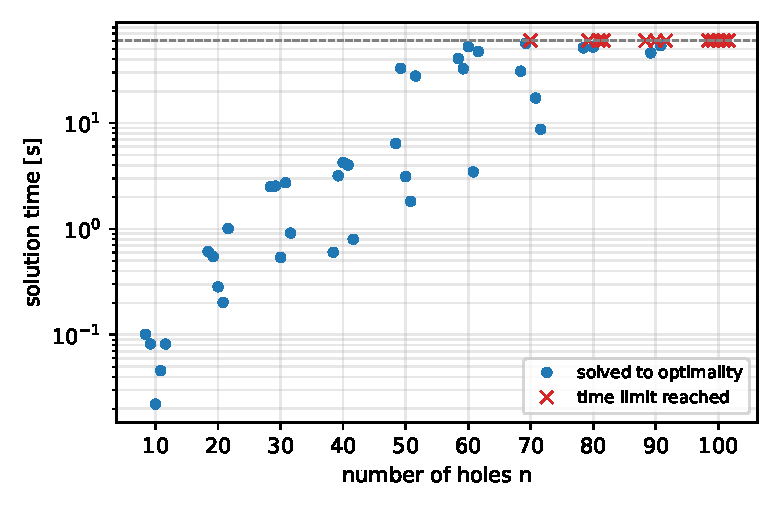
\includegraphics[width=0.7\textwidth]{figures/exact_time}
  \caption{Solution time of the exact method with the 60~s budget, one marker per instance
  (logarithmic scale). Crosses are the instances that reached the time limit.}
  \label{fig:time}
\end{figure}

\begin{figure}[htbp]\centering
  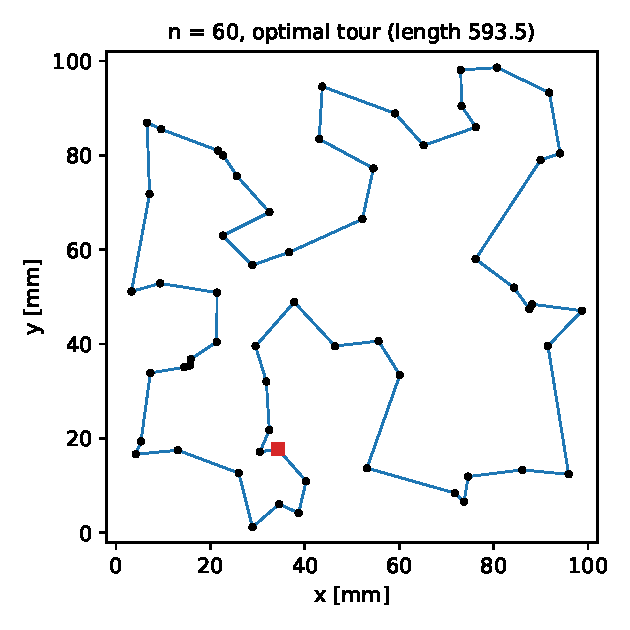
\includegraphics[width=0.55\textwidth]{figures/tour_n60}
  \caption{Optimal drilling sequence for instance \texttt{tsp\_n60\_1}, found by the exact
  method in 25~s (the square marks hole~0).}
  \label{fig:tour}
\end{figure}

\small
\begin{longtable}{lrrrrrrr}
\caption{Part I, every instance: best known value (optimum when proved), solution time in seconds when solved within the budget, otherwise the relative gap in parentheses; branch-and-bound nodes of the 60 s run.}\label{tab:p1inst}\\
\toprule
instance & $n$ & best known & 0.1 s & 1 s & 10 s & 60 s & nodes \\
\midrule
\endfirsthead
\toprule
instance & $n$ & best known & 0.1 s & 1 s & 10 s & 60 s & nodes \\
\midrule
\endhead
tsp\_n10\_1 & 10 & 235.3 & 0.04 & 0.04 & 0.10 & 0.10 & 0 \\
tsp\_n10\_2 & 10 & 265.2 & 0.05 & 0.04 & 0.08 & 0.08 & 0 \\
tsp\_n10\_3 & 10 & 301.1 & 0.01 & 0.01 & 0.03 & 0.02 & 0 \\
tsp\_n10\_4 & 10 & 274.5 & 0.03 & 0.02 & 0.04 & 0.05 & 0 \\
tsp\_n10\_5 & 10 & 275.2 & 0.05 & 0.03 & 0.08 & 0.08 & 0 \\
tsp\_n20\_1 & 20 & 419.7 & (66\%) & 0.29 & 0.62 & 0.61 & 0 \\
tsp\_n20\_2 & 20 & 442.5 & (61\%) & 0.25 & 0.53 & 0.55 & 124 \\
tsp\_n20\_3 & 20 & 340.6 & (64\%) & 0.13 & 0.27 & 0.28 & 0 \\
tsp\_n20\_4 & 20 & 345.6 & (68\%) & 0.10 & 0.19 & 0.20 & 0 \\
tsp\_n20\_5 & 20 & 418.5 & (61\%) & 0.43 & 0.99 & 1.01 & 0 \\
tsp\_n30\_1 & 30 & 469.4 & (68\%) & (1\%) & 2.58 & 2.51 & 127 \\
tsp\_n30\_2 & 30 & 473.6 & (74\%) & (3\%) & 2.50 & 2.54 & 234 \\
tsp\_n30\_3 & 30 & 414.3 & (73\%) & 0.21 & 0.54 & 0.54 & 0 \\
tsp\_n30\_4 & 30 & 439.1 & (72\%) & (0\%) & 2.76 & 2.73 & 17 \\
tsp\_n30\_5 & 30 & 460.0 & (70\%) & 0.38 & 0.88 & 0.91 & 0 \\
tsp\_n40\_1 & 40 & 532.9 & (80\%) & 0.24 & 0.60 & 0.60 & 0 \\
tsp\_n40\_2 & 40 & 526.4 & (76\%) & (23\%) & 3.25 & 3.17 & 0 \\
tsp\_n40\_3 & 40 & 552.9 & (76\%) & (10\%) & 4.30 & 4.24 & 34 \\
tsp\_n40\_4 & 40 & 499.9 & (79\%) & (17\%) & 4.05 & 4.02 & 44 \\
tsp\_n40\_5 & 40 & 516.9 & (77\%) & 0.34 & 0.77 & 0.80 & 0 \\
tsp\_n50\_1 & 50 & 554.8 & (100\%) & (11\%) & 6.41 & 6.42 & 23 \\
tsp\_n50\_2 & 50 & 554.5 & (85\%) & (80\%) & (17\%) & 32.95 & 593 \\
tsp\_n50\_3 & 50 & 571.9 & (80\%) & (9\%) & 3.02 & 3.12 & 23 \\
tsp\_n50\_4 & 50 & 614.1 & (100\%) & 0.79 & 1.81 & 1.82 & 12 \\
tsp\_n50\_5 & 50 & 585.2 & (83\%) & (81\%) & (37\%) & 27.79 & 538 \\
tsp\_n60\_1 & 60 & 593.5 & (100\%) & (82\%) & (62\%) & 40.74 & 736 \\
tsp\_n60\_2 & 60 & 647.0 & (100\%) & (81\%) & (17\%) & 32.51 & 505 \\
tsp\_n60\_3 & 60 & 588.5 & (100\%) & (82\%) & (25\%) & 52.65 & 505 \\
tsp\_n60\_4 & 60 & 630.4 & (100\%) & (80\%) & 3.51 & 3.46 & 0 \\
tsp\_n60\_5 & 60 & 606.9 & (100\%) & (83\%) & (15\%) & 47.36 & 776 \\
tsp\_n70\_1 & 70 & 655.2 & (100\%) & (84\%) & (5\%) & 30.90 & 1448 \\
tsp\_n70\_2 & 70 & 656.6 & (100\%) & (84\%) & (18\%) & 56.60 & 1435 \\
tsp\_n70\_3 & 70 & 671.1$^*$ & (100\%) & (84\%) & (47\%) & (47\%) & 299 \\
tsp\_n70\_4 & 70 & 636.9 & (100\%) & (85\%) & (0\%) & 17.23 & 1186 \\
tsp\_n70\_5 & 70 & 660.4 & (100\%) & (82\%) & 4.65 & 8.74 & 25 \\
tsp\_n80\_1 & 80 & 697.5 & (100\%) & (100\%) & (25\%) & 51.34 & 549 \\
tsp\_n80\_2 & 80 & 706.6$^*$ & (100\%) & (100\%) & (48\%) & (6\%) & 508 \\
tsp\_n80\_3 & 80 & 719.1 & (100\%) & (100\%) & (82\%) & 52.26 & 1878 \\
tsp\_n80\_4 & 80 & 710.6$^*$ & (100\%) & (100\%) & (84\%) & (11\%) & 470 \\
tsp\_n80\_5 & 80 & 668.0$^*$ & (100\%) & (100\%) & (81\%) & (8\%) & 470 \\
tsp\_n90\_1 & 90 & 740.7$^*$ & (100\%) & (100\%) & (86\%) & (7\%) & 951 \\
tsp\_n90\_2 & 90 & 698.1 & (100\%) & (100\%) & (85\%) & 45.98 & 515 \\
tsp\_n90\_3 & 90 & 741.5$^*$ & (100\%) & (100\%) & (87\%) & (15\%) & 515 \\
tsp\_n90\_4 & 90 & 756.9 & (100\%) & (100\%) & (86\%) & 53.75 & 515 \\
tsp\_n90\_5 & 90 & 737.0$^*$ & (100\%) & (100\%) & (84\%) & (33\%) & 515 \\
tsp\_n100\_1 & 100 & 787.5$^*$ & (100\%) & (100\%) & (88\%) & (7\%) & 457 \\
tsp\_n100\_2 & 100 & 791.6$^*$ & (100\%) & (100\%) & (86\%) & (12\%) & 480 \\
tsp\_n100\_3 & 100 & 770.3$^*$ & (100\%) & (100\%) & (87\%) & (4\%) & 480 \\
tsp\_n100\_4 & 100 & 756.7$^*$ & (100\%) & (100\%) & (88\%) & (1\%) & 480 \\
tsp\_n100\_5 & 100 & 753.3$^*$ & (100\%) & (100\%) & (87\%) & (7\%) & 480 \\
\bottomrule
\end{longtable}

\normalsize

%=====================================================================
\section{Part II: tabu search}\label{sec:assignment2}
%=====================================================================
\subsection{Why a metaheuristic, and why tabu search}
Part~I showed that the exact method is limited to boards of a few tens of holes, while a real
panel can easily have a hundred or more. When a proof of optimality is not needed, and it is
not needed on a production line, a heuristic that returns a very good tour in a fraction of a
second is the more useful tool. Among the metaheuristics seen in the course I chose tabu
search, for three reasons. It is a neighbourhood search, so it can exploit the structure of
the TSP: the 2-opt neighbourhood can be evaluated incrementally in constant time per move,
something a population-based method such as a genetic algorithm cannot do. It handles the
main weakness of local search, getting stuck in a local optimum, with a mechanism, the tabu
memory, that is simple to implement and has few parameters. And it is deterministic given the
random seed, which makes experiments reproducible.

Tabu search is a local search that always moves to the best neighbour of the current
solution, even when it is worse, and keeps a short-term memory of the recent moves, the
\emph{tabu list}, to avoid immediately undoing them and cycling between the same solutions.
The rest of this section describes how each component of the method was instantiated for the
TSP, the design decisions that were taken and the reasons for them.

\subsection{Design}\label{sec:design}
\paragraph{Solution representation.}
A tour is stored as the sequence of the $n$ holes in visiting order, \texttt{tour[0..n-1]}
(the \emph{path representation}), with the return arc from \texttt{tour[n-1]} to
\texttt{tour[0]} implicit. Together with it I keep the inverse map \texttt{pos[h]}, the
position of hole $h$ in the sequence, so that a hole can be located in $O(1)$.

\paragraph{Initial solution.}
The nearest neighbour heuristic: start from a random hole, always move to the closest hole
not yet visited, and close the cycle when all holes are visited. It costs $O(n^2)$ and gives a
tour typically 20--25\% longer than the optimum, with a few long arcs at the end where the
last holes left are far from each other. The search can also start from a random permutation;
the calibration (Section~\ref{sec:calib}) shows that the difference disappears after the
first iterations.

\paragraph{Neighbourhood.}
I use the 2-opt neighbourhood. A 2-opt move removes two non-adjacent arcs of the tour, say
$(a,b)$ and $(c,d)$ where $b$ follows $a$ and $d$ follows $c$, and reconnects the two paths
that remain in the only other way that gives a tour: with the arcs $(a,c)$ and $(b,d)$. In the
path representation the move is the \emph{reversal} of the sub-sequence that goes from $b$ to
$c$:
\[
  \langle \dots,a,\underbrace{b,\dots,c}_{\text{reversed}},d,\dots\rangle
  \;\longrightarrow\;
  \langle \dots,a,c,\dots,b,d,\dots\rangle .
\]
There is one move for every pair of non-adjacent arcs, $(n-1)(n-2)/2=O(n^2)$ moves in total:
4\,851 at $n=100$. Since the costs are symmetric the reversed sub-path costs exactly as
before, so the change of tour length caused by the move depends only on the four arcs
involved and is computed in $O(1)$:
\[
  \Delta = c_{ac} + c_{bd} - c_{ab} - c_{cd}.
\]
The whole neighbourhood is therefore evaluated in $O(n^2)$ operations. Applying the chosen
move, i.e.\ reversing the sub-sequence and updating \texttt{pos}, costs $O(n)$.

\paragraph{Exploration strategy.}
Steepest descent, or best improvement: at every iteration all the moves are evaluated and the
best \emph{admissible} one is applied, admissible meaning not tabu or satisfying the
aspiration criterion. The best move is applied even when its $\Delta$ is positive, i.e.\ when
it makes the tour longer: this is what allows the search to leave a local optimum.

\paragraph{Tabu memory.}
The purpose of the memory is to prevent the search, once it has climbed out of a local
optimum by a worsening move, from immediately stepping back into it. Storing the last visited
tours and comparing every neighbour with them would be expensive; the standard solution is to
store an \emph{attribute} of the recent moves. My attribute is the pair of arcs \emph{removed}
by a move: for \emph{tenure} iterations they may not be re-inserted in the tour. A move is
tabu if either of the two arcs it adds, $(a,c)$ or $(b,d)$, is currently tabu. The memory is
an $n\times n$ matrix \texttt{tabuUntil[u][v]}, symmetric, holding the number of the
iteration until which the arc $\{u,v\}$ is tabu; the check and the update are both $O(1)$. The
tenure is proportional to the size of the instance, $\max(5,\,0.125\,n)$, so that the same
rule applies to every board and no per-instance tuning is needed. Like any attribute-based
memory, this also forbids some moves that would lead to tours never visited (any tour
containing a tabu arc), which is the price of a cheap memory; the aspiration criterion
repairs the cases that matter.

\paragraph{Aspiration criterion.}
A tabu move is accepted anyway if it leads to a tour shorter than the best tour found so far.
Such a tour cannot have been visited before (it is better than everything visited), so
accepting it cannot cause cycling, and refusing it would mean discarding the best solution
just because of the bookkeeping of the memory.

\paragraph{Diversification.}
Tabu search alone explores the region around the current solution well, but after a while it
tends to circle in the same area: the tabu list only forbids short cycles. A diversification
mechanism is needed to move the search to a different region of the solution space. Mine is
the \emph{kick} (the ``kick search'' of the course notes: use the normal neighbourhood, and
occasionally apply a larger move to jump elsewhere): when no improvement of the best tour has been found for $0.5\,n$ consecutive
iterations, the search is considered stuck; the best tour is copied, perturbed with $k=6$
random \emph{double-bridge} moves, and the search restarts from the perturbed tour with an
empty tabu memory. A double bridge cuts the tour into four segments $A\,B\,C\,D$ (three random
cut points) and reconnects them as $A\,C\,B\,D$; it changes four arcs, it is cheap ($O(n)$)
and, most important, it cannot be undone by a single 2-opt move, so the search does not simply
fall back into the local optimum it came from. This is the classical perturbation used with
2-opt in the literature (it is the kick of the iterated Lin--Kernighan and of many ``iterated
local search'' methods).

\paragraph{Stopping criterion.}
A time limit, the same budgets as Part~I, so that the two methods can be compared at equal
time; or an iteration limit, used in the calibration. When the search stops, the best tour
found is returned.

\paragraph{The algorithm.}
Putting the components together:
\begin{enumerate}[nosep]
  \item build the initial tour $s$ (nearest neighbour); $s^*\leftarrow s$; clear the memory;
  \item repeat until the stopping criterion holds:
  \begin{enumerate}[nosep]
    \item scan all 2-opt moves of $s$; keep the one with the smallest $\Delta$ among those not
      tabu or leading to a tour better than $s^*$;
    \item if no move is admissible, clear the memory and go to (a);
    \item mark the two removed arcs tabu until iteration $t+\text{tenure}$; apply the move;
    \item if $s$ is better than $s^*$: $s^*\leftarrow s$, reset the idle counter; otherwise
      increment it;
    \item if the idle counter reaches $0.5\,n$: $s\leftarrow$ double-bridge$^k(s^*)$, clear
      the memory, reset the counter;
  \end{enumerate}
  \item return $s^*$.
\end{enumerate}

\subsection{Implementation}\label{sec:impl2}
The search is implemented in the class \texttt{TabuSearch}, files \texttt{tabu\_search.h} and
\texttt{tabu\_search.cpp} in \texttt{assignment\_2/}; it needs no library besides the C++ standard
one. The cost matrix is
copied into a flat array of doubles, \texttt{c[i*n+j]}, for locality; the tabu matrix is a
flat array of iteration numbers of the same shape. The core of an iteration is the scan of the
neighbourhood:
\begin{lstlisting}
for (int i = 0; i < n_ - 2; ++i) {
    int a = tour_[i], b = tour_[i + 1];
    double cab = c(a, b);
    int jmax = (i == 0) ? n_ - 2 : n_ - 1;      // the two removed arcs must not be adjacent
    for (int j = i + 2; j <= jmax; ++j) {
        int cc = tour_[j], d = tour_[j + 1 == n_ ? 0 : j + 1];
        double delta = c(a, cc) + c(b, d) - cab - c(cc, d);
        if (delta >= bestDelta) continue;        // not better than the best move so far
        bool tabuMove = isTabu(a, cc, iter) || isTabu(b, d, iter);
        if (tabuMove && !(cost_ + delta < bestCost - 1e-9)) continue;   // aspiration
        bestDelta = delta; bi = i; bj = j;
    }
}
\end{lstlisting}
Note the order of the two tests: the tabu status is checked only for moves that would improve
on the best move found so far in this scan, which are few, so the memory is consulted rarely.
Every iteration costs $O(n^2)$ for the scan plus $O(n)$ for the reversal; on the test machine
the search performs about $120\,000$ iterations per second at $n=100$, $470\,000$ at $n=50$ and
more than a million at $n=30$. The random generator (\texttt{std::mt19937}) is seeded from the
command line, so every run is reproducible; the same seed gives the same tour on any machine,
as I verified on the laboratory computer.

\subsection{Design issues}\label{sec:issues}
Some choices deserve a justification, because they were made after considering, and in some
cases trying, the alternative.

\paragraph{Arc-based rather than node-based tabu attribute.}
A cheaper memory stores, for every hole, the last iteration in which it was an endpoint of a
move, and declares a move tabu if its holes were touched recently; it needs a vector instead
of a matrix. I preferred the removed arcs because of what is forbidden. With arcs, only the
moves that re-insert an arc just removed, and in particular the move that undoes the last one,
are tabu: this is exactly the cycling to prevent, and nothing else. With holes, every
move touching those holes is forbidden, including many unrelated ones, so the memory has to be
short to leave enough admissible moves, and the search is constrained where it should not be.
The price, an $n\times n$ matrix of integers, is negligible next to the cost matrix.

\paragraph{Full scan instead of first improvement.}
A first-improvement strategy applies the first improving move found and saves the rest of the
scan. It is attractive early in the search, when improving moves are plentiful, but it saves
nothing at a local optimum, where every move must be examined to conclude that none improves,
and local optima are exactly where a tabu search spends its time. With the $O(1)$ evaluation
a full scan costs a few microseconds at $n=100$, so I always take the best move; this also
makes the trajectory deterministic given the seed.

\paragraph{Why 2-opt and not 3-opt.}
The 3-opt neighbourhood has $O(n^3)$ moves, a thousand times more at $n=100$, and several
ways to reconnect the three paths, for a modest gain in the quality of local optima. I kept
the cheap neighbourhood and obtain the larger moves from the kicks: a double bridge is itself
a 4-opt move, applied only when the search stalls and at a cost of $O(n)$. The calibration
confirms that this combination reaches the optimum of the calibration instances in every
run.

\paragraph{Restart from the best tour, with an empty memory.}
After a kick the search restarts from a perturbed copy of the \emph{best} tour rather than of
the current one. The current tour, after $0.5\,n$ non-improving iterations, may have drifted
to a mediocre region; the best tour is a proven good starting point, and the kicks make sure
the search does not repeat the same trajectory from it. Clearing the tabu memory at the
restart is necessary because the stored arcs refer to the tour before the kick.

\paragraph{Real-valued costs and rounding.}
Because costs are floating-point numbers, the tour length tracked incrementally by adding the
$\Delta$ of every move accumulates rounding errors over millions of iterations. Two measures
deal with this. The length is recomputed from scratch whenever a new best tour is found, an
$O(n)$ operation that happens rarely; and the comparisons ``better than the best'' use a small
tolerance ($10^{-9}$), so that a move is not accepted as improving because of rounding noise.
At the end the program recomputes the length of the returned tour independently and checks it
against the value tracked by the search, and it also checks that the tour visits every hole
exactly once.

\paragraph{Empty neighbourhood.}
If every move were tabu and none satisfied the aspiration criterion, the search would have no
admissible move. With a tenure of $0.125\,n$ and a neighbourhood of $O(n^2)$ moves this never
happened in my runs, but the code handles the case by clearing the memory and repeating the
iteration, rather than stopping.

\paragraph{Small instances.}
The double bridge needs at least eight holes to cut the tour into four non-empty segments;
below that the perturbation is a random shuffle. For $n\le40$ the tenure floor of 5
iterations applies ($0.125\,n\le5$): a tenure below a handful of iterations would not even
prevent the shortest cycles.

\subsection{Calibration}\label{sec:calib}
The tabu search has four parameters: the tabu tenure, the number of idle iterations before a
kick, the strength of the kick (number of double-bridge moves) and the choice of the initial
solution. Their calibration is a pre-deployment activity: the values are chosen once, on the
calibration instances, and then used unchanged on every benchmark instance. Since the
parameters are expressed as fractions of $n$, the same rule applies to every size.

\paragraph{Protocol.}
Every configuration was run on the eight calibration instances with five seeds each (40 runs
per configuration) and a budget of $50\,000$ iterations. Using an iteration budget instead of
a time limit makes all configurations do exactly the same amount of work, so the comparison
does not depend on the load of the machine or on the speed of the computer. I varied one
parameter at a time around a starting configuration (tenure $0.125\,n$, kick after $n$ idle
iterations, 6 double bridges, nearest-neighbour start), which is a rough but sufficient
tuning for four parameters. The quality measure is the percentage gap to the best known value
of the instance: the optimum proved by CPLEX in 60~s (all the instances with $n\le50$ and one
with $n=70$), and the best tour found by any run otherwise. Table~\ref{tab:calib} reports,
for every configuration, the mean gap over the 40 runs, its standard deviation, the worst run,
the average iteration at which the best tour was found and the average running time.

\begin{table}[htbp]\centering\small
\caption{Calibration of the tabu search (8 instances $\times$ 5 seeds per configuration,
$50\,000$ iterations each). Gap in \% to the best known value: mean over the 40 runs,
standard deviation and worst run; average iteration at which the best tour was found.}
\label{tab:calib}
\begin{tabular}{llrrrrr}
\toprule
config. & description & mean gap & std & worst & it. to best & time (s) \\
\midrule
kick0 & no kicks (plain tabu search) & 3.771 & 2.632 & 10.88 & 19 & 0.00 \\
kick1 & 1 double bridge & 0.232 & 0.463 & 1.92 & 8710 & 0.41 \\
kick3 & 3 double bridges & 0.045 & 0.165 & 0.82 & 7003 & 0.42 \\
kick6 & 6 double bridges (default) & 0.007 & 0.040 & 0.25 & 9194 & 0.42 \\
wait0.5 & kick after $0.5n$ idle it. & 0.000 & 0.000 & 0.00 & 5408 & 0.41 \\
wait2 & kick after $2n$ idle it. & 0.070 & 0.175 & 0.66 & 10799 & 0.43 \\
wait5 & kick after $5n$ idle it. & 0.142 & 0.267 & 0.95 & 10810 & 0.27 \\
ten0.05 & tenure $0.05n$ & 0.039 & 0.184 & 1.07 & 4129 & 0.22 \\
ten0.25 & tenure $0.25n$ & 0.012 & 0.075 & 0.47 & 5833 & 0.25 \\
ten0.5 & tenure $0.5n$ & 0.048 & 0.154 & 0.66 & 7328 & 0.31 \\
random & random initial tour & 0.043 & 0.164 & 0.82 & 4414 & 0.43 \\
\bottomrule
\end{tabular}

\end{table}

\paragraph{What the table says.}
\begin{itemize}
  \item \emph{Diversification is the parameter that matters.} Without kicks
    (\texttt{kick0}) the search stops after about 80 iterations, at the first local optimum it
    cannot leave: with only the tabu memory, once every neighbour of the local optimum has
    been tried, the search wanders in its basin and never finds anything better. The gap is
    3.8\% on average and 11\% in the worst run. One double bridge brings the gap to 0.23\%,
    three to 0.05\%, six to 0.007\%: a stronger perturbation moves the search further and
    is better, up to the point where the tour is essentially reshuffled. Kicking earlier is
    also better: waiting $0.5\,n$ idle iterations instead of $n$ reaches the best known value
    in every run, while waiting $5\,n$ leaves 0.14\% and wastes iterations in a region the
    search has already exhausted.
  \item \emph{The tenure has a minor effect.} Between $0.05\,n$ and $0.5\,n$ the average gap
    stays between 0.01\% and 0.05\%, all within one standard deviation of each other. This is
    consistent with the role of the tabu list in this design: it only has to prevent short
    cycles around the current tour, while the exploration of distant regions is done by the
    kicks. A very long tenure ($0.5\,n$) is slightly worse, as it forbids too many moves.
  \item \emph{The initial solution does not matter.} Starting from a random tour instead of
    the nearest-neighbour tour gives 0.04\% instead of 0.007\%, and the best tour is found
    at an earlier iteration on average. The first improving iterations of the search repair
    a bad start in a few hundred moves, so the quality of the starting tour has no lasting
    influence, which is what the course notes warn: a better initial solution does not
    guarantee a better final one.
\end{itemize}
The final configuration is therefore tenure $\max(5,\,0.125\,n)$, a kick of 6 double bridges
after $0.5\,n$ iterations without improvement, nearest-neighbour start. These are the default
values of the program.

\subsection{Results}\label{sec:p2results}
The tabu search was run on the 50 benchmark instances with the same time budgets as the exact
method: 0.1~s and 1~s with 10 seeds per instance, 10~s with 5 seeds, 1\,250 runs in total.
The reference value of every instance is its \emph{best known value}: the optimum proved by
CPLEX for the 38 instances solved in 60~s, and the best tour found by any run (of any method
and budget) for the other 12; for these, Section~\ref{sec:p1results} showed that the CPLEX
lower bound is within 1.2\% on average, so a gap of zero to the best known value means a tour
within about one percent of the optimum. Since the search is stochastic, I report
statistics over the seeds: Table~\ref{tab:p2} gives for every size and budget the mean and the
standard deviation of the gap over all runs, the average over the instances of the worst
run, and the percentage of runs that reached the best known value; Table~\ref{tab:p2inst}
gives the mean and the worst gap of every single instance. Figure~\ref{fig:gap} plots the mean
gap against the size.

\begin{table}[htbp]\centering\small
\caption{Part II, summary by size: gap (\%) of the tabu search to the best known value, mean
and standard deviation over all runs, average over the instances of the worst run, and
percentage of runs that reached the best known value. 10 seeds per instance at 0.1 and 1~s,
5 seeds at 10~s.}
\label{tab:p2}
\begin{tabular}{rcccccccccccc}
\toprule
& \multicolumn{4}{c}{0.1 s} & \multicolumn{4}{c}{1 s} & \multicolumn{4}{c}{10 s} \\
\cmidrule(lr){2-5} \cmidrule(lr){6-9} \cmidrule(lr){10-13}
$n$ & mean & std & worst & hits& mean & std & worst & hits& mean & std & worst & hits \\
\midrule
10 & 0.00 & 0.00 & 0.00 & 100\% & 0.00 & 0.00 & 0.00 & 100\% & 0.00 & 0.00 & 0.00 & 100\% \\
20 & 0.00 & 0.00 & 0.00 & 100\% & 0.00 & 0.00 & 0.00 & 100\% & 0.00 & 0.00 & 0.00 & 100\% \\
30 & 0.00 & 0.00 & 0.00 & 100\% & 0.00 & 0.00 & 0.00 & 100\% & 0.00 & 0.00 & 0.00 & 100\% \\
40 & 0.00 & 0.00 & 0.00 & 100\% & 0.00 & 0.00 & 0.00 & 100\% & 0.00 & 0.00 & 0.00 & 100\% \\
50 & 0.00 & 0.00 & 0.00 & 100\% & 0.00 & 0.00 & 0.00 & 100\% & 0.00 & 0.00 & 0.00 & 100\% \\
60 & 0.00 & 0.03 & 0.04 & 98\% & 0.00 & 0.00 & 0.00 & 100\% & 0.00 & 0.00 & 0.00 & 100\% \\
70 & 0.07 & 0.21 & 0.19 & 88\% & 0.00 & 0.00 & 0.00 & 100\% & 0.00 & 0.00 & 0.00 & 100\% \\
80 & 0.18 & 0.35 & 0.66 & 56\% & 0.00 & 0.00 & 0.00 & 96\% & 0.00 & 0.00 & 0.00 & 100\% \\
90 & 0.15 & 0.26 & 0.56 & 60\% & 0.00 & 0.00 & 0.00 & 100\% & 0.00 & 0.00 & 0.00 & 100\% \\
100 & 0.52 & 0.62 & 1.72 & 26\% & 0.05 & 0.13 & 0.22 & 70\% & 0.02 & 0.08 & 0.06 & 88\% \\
\bottomrule
\end{tabular}

\end{table}

\begin{figure}[htbp]\centering
  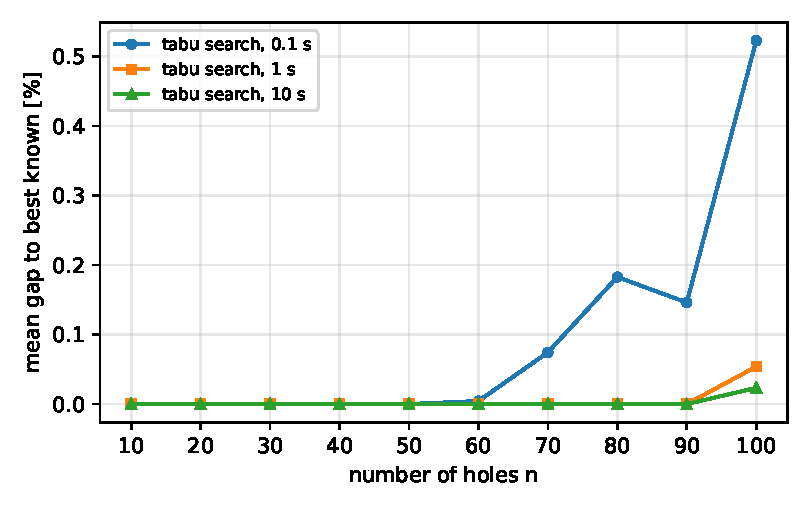
\includegraphics[width=0.7\textwidth]{figures/tabu_gap}
  \caption{Mean gap of the tabu search to the best known value as a function of the size, for
  the three time budgets.}
  \label{fig:gap}
\end{figure}

With \textbf{0.1~s} the tabu search returns the optimum in every run for every instance up to
50 holes; recall that the exact method with the same budget proves optimality only at 10
holes. Beyond 50 holes the mean gap grows slowly, to 0.5\% at $n=100$, where a quarter of the
runs still reach the best known value and the worst run is 1.7\% off: with 0.1~s the search
performs only about $5\,000$ iterations at $n=100$, roughly a hundred kicks, and that is not
always enough to find the last improvements. With \textbf{1~s} the gap is zero, in every run,
up to 90 holes (a single run out of fifty at $n=80$ is 0.002\% off) and 0.05\% at $n=100$, with
70\% of the runs at the best known value. The best tour is found after 0.13~s on average at
$n=100$ and after a few milliseconds below $n=60$, so most of the budget is spent confirming
the result. With \textbf{10~s} the only non-zero entry of the table is 0.02\% at $n=100$, with
88\% of the runs reaching the best known value. The standard deviations show that the method
is reliable: at 1~s the spread between seeds is nil up to $n=90$ and 0.13\% at $n=100$.

Figure~\ref{fig:n100} shows what these numbers mean on a 100-hole board: the tour returned
by CPLEX after 60~s still has many crossing arcs (a tour with a crossing is never optimal
in the Euclidean plane, since uncrossing it is a 2-opt move that shortens it), the tabu tour
after one second has none.

\begin{figure}[htbp]\centering
  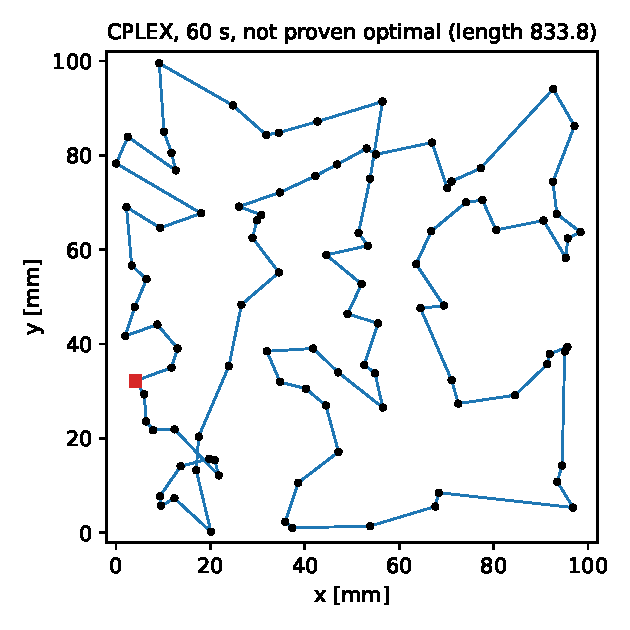
\includegraphics[width=0.48\textwidth]{figures/tour_n100_cplex}\hfill
  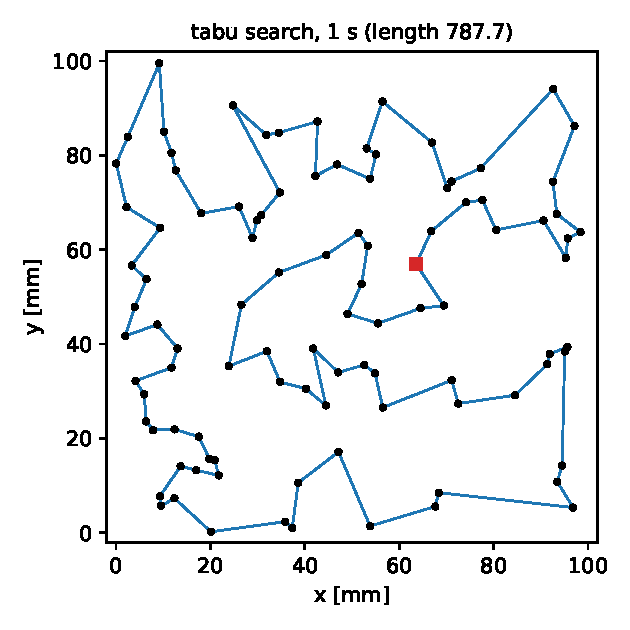
\includegraphics[width=0.48\textwidth]{figures/tour_n100_tabu}
  \caption{Instance \texttt{tsp\_n100\_1}: incumbent of the exact method after 60~s (left,
  gap 7.0\% to its own bound, 5.9\% longer than the tour on the right) and tour of the tabu
  search after 1~s (right, the best known value for this instance).}
  \label{fig:n100}
\end{figure}

\subsection{Comparison with the exact method}\label{sec:compare}
Table~\ref{tab:h2h} puts the two methods side by side at equal time budget: for every size
and budget, the number of instances CPLEX solved to optimality, the average gap of the CPLEX
incumbent to the best known value, and the average gap of the tabu search.

\begin{table}[htbp]\centering\small
\caption{Exact method and tabu search at the same time budget: instances CPLEX solved to
optimality, average gap (\%) of the CPLEX incumbent to the best known value, and average gap
(\%) of the tabu search.}
\label{tab:h2h}
\resizebox{\textwidth}{!}{\begin{tabular}{rccccccccc}
\toprule
& \multicolumn{3}{c}{0.1 s} & \multicolumn{3}{c}{1 s} & \multicolumn{3}{c}{10 s} \\
\cmidrule(lr){2-4} \cmidrule(lr){5-7} \cmidrule(lr){8-10}
$n$ & CPLEX opt. & CPLEX gap & TS gap& CPLEX opt. & CPLEX gap & TS gap& CPLEX opt. & CPLEX gap & TS gap \\
\midrule
10 & 5/5 & 0.0 & 0.00 & 5/5 & 0.0 & 0.00 & 5/5 & 0.0 & 0.00 \\
20 & 0/5 & 162.4 & 0.00 & 5/5 & 0.0 & 0.00 & 5/5 & 0.0 & 0.00 \\
30 & 0/5 & 209.3 & 0.00 & 2/5 & 0.5 & 0.00 & 5/5 & 0.0 & 0.00 \\
40 & 0/5 & 282.0 & 0.00 & 2/5 & 11.7 & 0.00 & 5/5 & 0.0 & 0.00 \\
50 & 0/5 & 359.1 & 0.00 & 1/5 & 157.0 & 0.00 & 3/5 & 13.3 & 0.00 \\
60 & 0/5 & 419.8 & 0.00 & 0/5 & 419.8 & 0.00 & 1/5 & 43.2 & 0.00 \\
70 & 0/5 & 443.3 & 0.07 & 0/5 & 443.3 & 0.00 & 1/5 & 21.5 & 0.00 \\
80 & 0/5 & 460.8 & 0.18 & 0/5 & 460.8 & 0.00 & 0/5 & 286.0 & 0.00 \\
90 & 0/5 & 517.1 & 0.15 & 0/5 & 517.1 & 0.00 & 0/5 & 517.1 & 0.00 \\
100 & 0/5 & 575.0 & 0.52 & 0/5 & 575.0 & 0.05 & 0/5 & 575.0 & 0.02 \\
\bottomrule
\end{tabular}
}
\end{table}

Three observations summarise the comparison.
\begin{itemize}
  \item \emph{Where CPLEX proves optimality, the tabu search finds the same value}, in every
    run, and much faster: the 40-hole instances need 2.6~s of CPLEX and a few milliseconds of
    tabu search.
  \item \emph{Where CPLEX runs out of time, its incumbent is far from the best known tour}:
    12\% at $n=40$ with 1~s, 43\% at $n=60$ with 10~s, and several times the optimal length
    with 0.1~s, while the tabu search stays within a fraction of a percent. The incumbent of a
    truncated branch-and-bound is whatever the internal heuristics of the solver happened to
    find; it is not a good tour, and a user with a tenth of a second and this model would
    have nothing usable to give to the machine.
  \item \emph{On no instance and no budget is the CPLEX incumbent better than the tabu
    search.} This is also true at 60~s: none of the 12 incumbents of the instances not closed
    in 60~s beats the tabu tour found in 10~s, and on average they are 17\% longer.
\end{itemize}
Is it better to use the heuristic or the mathematical programming model? For the drilling
application the answer is the heuristic: a board of a hundred holes is sequenced within a
fraction of a percent of the optimum in a second, and a proof of optimality has no value for
the machine operator. The exact method keeps two roles. It is the right tool when a proof is
needed and the board is small, up to 40--60 holes with a budget of 10--60~s; and even when
it cannot close an instance it provides a lower bound, which is what allowed me to state that
the heuristic tours on the largest boards are within a few percent of the optimum. The two
methods are complementary: the exact one certifies the heuristic on the sizes it can handle,
the heuristic extends the reach to the sizes the exact one cannot.

\small
\begin{longtable}{lrrrrrrrr}
\caption{Part II, every instance: gap (\%) to the best known value of the mean and of the worst run, for each budget, and average time (s) at which the best tour of the 1 s runs was found.}\label{tab:p2inst}\\
\toprule
 & & \multicolumn{2}{c}{0.1 s} & \multicolumn{3}{c}{1 s} & \multicolumn{2}{c}{10 s} \\
\cmidrule(lr){3-4}\cmidrule(lr){5-7}\cmidrule(lr){8-9}
instance & best known & mean & worst & mean & worst & $t_{best}$ & mean & worst \\
\midrule
\endfirsthead
\toprule
instance & best known & mean & worst & mean & worst & $t_{best}$ & mean & worst \\
\midrule
\endhead
tsp\_n10\_1 & 235.3 & 0.00 & 0.00 & 0.00 & 0.00 & 0.000 & 0.00 & 0.00 \\
tsp\_n10\_2 & 265.2 & 0.00 & 0.00 & 0.00 & 0.00 & 0.000 & 0.00 & 0.00 \\
tsp\_n10\_3 & 301.1 & 0.00 & 0.00 & 0.00 & 0.00 & 0.000 & 0.00 & 0.00 \\
tsp\_n10\_4 & 274.5 & 0.00 & 0.00 & 0.00 & 0.00 & 0.000 & 0.00 & 0.00 \\
tsp\_n10\_5 & 275.2 & 0.00 & 0.00 & 0.00 & 0.00 & 0.000 & 0.00 & 0.00 \\
tsp\_n20\_1 & 419.7 & 0.00 & 0.00 & 0.00 & 0.00 & 0.000 & 0.00 & 0.00 \\
tsp\_n20\_2 & 442.5 & 0.00 & 0.00 & 0.00 & 0.00 & 0.000 & 0.00 & 0.00 \\
tsp\_n20\_3 & 340.6 & 0.00 & 0.00 & 0.00 & 0.00 & 0.000 & 0.00 & 0.00 \\
tsp\_n20\_4 & 345.6 & 0.00 & 0.00 & 0.00 & 0.00 & 0.000 & 0.00 & 0.00 \\
tsp\_n20\_5 & 418.5 & 0.00 & 0.00 & 0.00 & 0.00 & 0.000 & 0.00 & 0.00 \\
tsp\_n30\_1 & 469.4 & 0.00 & 0.00 & 0.00 & 0.00 & 0.001 & 0.00 & 0.00 \\
tsp\_n30\_2 & 473.6 & 0.00 & 0.00 & 0.00 & 0.00 & 0.000 & 0.00 & 0.00 \\
tsp\_n30\_3 & 414.3 & 0.00 & 0.00 & 0.00 & 0.00 & 0.000 & 0.00 & 0.00 \\
tsp\_n30\_4 & 439.1 & 0.00 & 0.00 & 0.00 & 0.00 & 0.000 & 0.00 & 0.00 \\
tsp\_n30\_5 & 460.0 & 0.00 & 0.00 & 0.00 & 0.00 & 0.000 & 0.00 & 0.00 \\
tsp\_n40\_1 & 532.9 & 0.00 & 0.00 & 0.00 & 0.00 & 0.000 & 0.00 & 0.00 \\
tsp\_n40\_2 & 526.4 & 0.00 & 0.00 & 0.00 & 0.00 & 0.002 & 0.00 & 0.00 \\
tsp\_n40\_3 & 552.9 & 0.00 & 0.00 & 0.00 & 0.00 & 0.001 & 0.00 & 0.00 \\
tsp\_n40\_4 & 499.9 & 0.00 & 0.00 & 0.00 & 0.00 & 0.001 & 0.00 & 0.00 \\
tsp\_n40\_5 & 516.9 & 0.00 & 0.00 & 0.00 & 0.00 & 0.000 & 0.00 & 0.00 \\
tsp\_n50\_1 & 554.8 & 0.00 & 0.00 & 0.00 & 0.00 & 0.002 & 0.00 & 0.00 \\
tsp\_n50\_2 & 554.5 & 0.00 & 0.00 & 0.00 & 0.00 & 0.004 & 0.00 & 0.00 \\
tsp\_n50\_3 & 571.9 & 0.00 & 0.00 & 0.00 & 0.00 & 0.001 & 0.00 & 0.00 \\
tsp\_n50\_4 & 614.1 & 0.00 & 0.00 & 0.00 & 0.00 & 0.002 & 0.00 & 0.00 \\
tsp\_n50\_5 & 585.2 & 0.00 & 0.00 & 0.00 & 0.00 & 0.004 & 0.00 & 0.00 \\
tsp\_n60\_1 & 593.5 & 0.00 & 0.00 & 0.00 & 0.00 & 0.009 & 0.00 & 0.00 \\
tsp\_n60\_2 & 647.0 & 0.00 & 0.00 & 0.00 & 0.00 & 0.010 & 0.00 & 0.00 \\
tsp\_n60\_3 & 588.5 & 0.00 & 0.00 & 0.00 & 0.00 & 0.002 & 0.00 & 0.00 \\
tsp\_n60\_4 & 630.4 & 0.00 & 0.00 & 0.00 & 0.00 & 0.004 & 0.00 & 0.00 \\
tsp\_n60\_5 & 606.9 & 0.02 & 0.22 & 0.00 & 0.00 & 0.014 & 0.00 & 0.00 \\
tsp\_n70\_1 & 655.2 & 0.34 & 0.69 & 0.00 & 0.00 & 0.088 & 0.00 & 0.00 \\
tsp\_n70\_2 & 656.6 & 0.00 & 0.00 & 0.00 & 0.00 & 0.009 & 0.00 & 0.00 \\
tsp\_n70\_3 & 671.1 & 0.03 & 0.28 & 0.00 & 0.00 & 0.020 & 0.00 & 0.00 \\
tsp\_n70\_4 & 636.9 & 0.00 & 0.00 & 0.00 & 0.00 & 0.005 & 0.00 & 0.00 \\
tsp\_n70\_5 & 660.4 & 0.00 & 0.00 & 0.00 & 0.00 & 0.007 & 0.00 & 0.00 \\
tsp\_n80\_1 & 697.5 & 0.02 & 0.05 & 0.00 & 0.00 & 0.044 & 0.00 & 0.00 \\
tsp\_n80\_2 & 706.6 & 0.13 & 0.53 & 0.00 & 0.00 & 0.176 & 0.00 & 0.00 \\
tsp\_n80\_3 & 719.1 & 0.06 & 0.59 & 0.00 & 0.01 & 0.024 & 0.00 & 0.00 \\
tsp\_n80\_4 & 710.6 & 0.31 & 0.89 & 0.00 & 0.00 & 0.079 & 0.00 & 0.00 \\
tsp\_n80\_5 & 668.0 & 0.40 & 1.21 & 0.00 & 0.00 & 0.055 & 0.00 & 0.00 \\
tsp\_n90\_1 & 740.7 & 0.10 & 0.30 & 0.00 & 0.00 & 0.062 & 0.00 & 0.00 \\
tsp\_n90\_2 & 698.1 & 0.00 & 0.00 & 0.00 & 0.00 & 0.016 & 0.00 & 0.00 \\
tsp\_n90\_3 & 741.5 & 0.30 & 1.14 & 0.00 & 0.00 & 0.164 & 0.00 & 0.00 \\
tsp\_n90\_4 & 756.9 & 0.05 & 0.54 & 0.00 & 0.00 & 0.031 & 0.00 & 0.00 \\
tsp\_n90\_5 & 737.0 & 0.27 & 0.83 & 0.00 & 0.00 & 0.151 & 0.00 & 0.00 \\
tsp\_n100\_1 & 787.5 & 0.34 & 1.29 & 0.03 & 0.10 & 0.322 & 0.00 & 0.02 \\
tsp\_n100\_2 & 791.6 & 0.44 & 1.39 & 0.17 & 0.28 & 0.052 & 0.11 & 0.28 \\
tsp\_n100\_3 & 770.3 & 0.34 & 1.92 & 0.00 & 0.00 & 0.039 & 0.00 & 0.00 \\
tsp\_n100\_4 & 756.7 & 0.43 & 1.74 & 0.00 & 0.00 & 0.064 & 0.00 & 0.00 \\
tsp\_n100\_5 & 753.3 & 1.07 & 2.29 & 0.07 & 0.71 & 0.168 & 0.00 & 0.00 \\
\bottomrule
\end{longtable}

\normalsize

%=====================================================================
\section{Environment and measurements}\label{sec:env}
%=====================================================================
\paragraph{Machines.}
All the experiments reported here were run on a laptop with an AMD Ryzen~7 5800H processor
(8 cores) and 13~GB of RAM, under Arch Linux, with g++~16.2 and CPLEX~22.2. The code was also
compiled and tested on the laboratory machine \texttt{labta} of the department (Debian~12, g++~12.2,
CPLEX~22.1.1), where it builds with the same Makefile without any change and returns
the same optima and the same tabu tours. The running times of the exact method are of the
same order but not identical, because the two CPLEX versions follow different
branch-and-bound paths: for instance \texttt{tsp\_n10\_1}, \texttt{tsp\_n30\_1} and
\texttt{tsp\_n60\_1} take 0.07, 1.6 and 6.8~s on \texttt{labta} against 0.07, 2.4 and
41~s on the laptop. The sizes reported in Section~\ref{sec:p1results} should therefore be
read as indicative for the laboratory computers, where the exact method is, if anything,
slightly faster.

\paragraph{Time measurements.}
Times are wall-clock times measured with the C++ \texttt{steady\_clock} around the call to
\texttt{CPXmipopt} (Part~I) or around the search loop (Part~II); the time needed to read
the instance, build the model and print the results is measured separately and not counted
in the budgets. Both programs are single-threaded, so wall-clock time and CPU time coincide,
and the time limits are wall-clock limits. The campaigns of Part~I with different budgets were
run as separate processes on different cores; at most two single-threaded processes were
active at the same time on the 8-core machine, so the runs did not compete for CPU.

\paragraph{Reproducibility.}
The instances are generated from fixed seeds, the tabu search is seeded from the command line
and CPLEX runs deterministically on one thread, so every number in this report can be
regenerated with the scripts in \texttt{scripts/} (see Section~\ref{sec:build}).

%=====================================================================
\section{Conclusions}\label{sec:concl}
%=====================================================================
The exercise asked up to which size the flow model of the TSP can be solved exactly in a
given time. On the benchmark of this report, with one thread and a strict reading (every
instance of a size solved), the answer is 10 holes in 0.1~s, 20 in 1~s, 40 in 10~s and 60 in
60~s, with single instances of up to 90 holes solved in 60~s. The limiting factor is the
branch-and-bound tree: from about 50 holes the linear relaxation of the flow model no longer
closes the gap at the root node, and the number of nodes, and with it the time, grows
exponentially with the size.

The tabu search of Part~II, with a 2-opt neighbourhood evaluated incrementally, an arc-based
tabu memory with aspiration and double-bridge kicks as diversification, reaches the optimum
of every instance up to 50 holes in 0.1~s and up to 90 holes in 1~s in every run, and stays
within 0.5\% of the best known value at 100 holes even with 0.1~s. The calibration showed
that the diversification mechanism, and not the tabu tenure or the initial solution, is
what decides the quality of the result: a plain tabu search without kicks stops at 3.8\% from
the optimum, the same search with kicks finds it. For the drilling application, where a board
with a hundred holes must be sequenced quickly and a proof of optimality has no practical
value, the heuristic is the method of choice; the exact method remains useful to certify the
heuristic on small boards and to provide the lower bounds that show how close the heuristic
tours are to the optimum on the large ones.

\paragraph{Possible improvements.}
On the exact side, the weakness of the model is the big-M linking constraint; a formulation
with subtour elimination constraints generated on demand (solve the relaxation, find a
violated subtour constraint, add it, repeat) has a much stronger relaxation and is what
state-of-the-art TSP codes use, at the price of a separation procedure. On the heuristic side,
the search could be made faster on large boards by restricting the 2-opt scan to the $k$
nearest neighbours of each hole (a \emph{granular} neighbourhood, $O(kn)$ instead of $O(n^2)$),
and richer moves such as Or-opt (moving a short segment elsewhere) could be added; on the
present benchmark, however, the search already returns optimal tours in a fraction of a
second, so these refinements would only matter for boards with several hundred holes.

%=====================================================================
\section{Building and running the code}\label{sec:build}
%=====================================================================
The code is C++11 and is built with the \texttt{Makefile} in the project root:
\texttt{make} builds both \texttt{tsp\_cplex} (Part~I) and \texttt{tsp\_tabu} (Part~II);
\texttt{make tsp\_tabu} builds Part~II alone, which does not need CPLEX. The Makefile uses the
CPLEX installation of the laboratory machines (\texttt{/opt/ibm/ILOG/CPLEX\_Studio2211}) if
present, otherwise the software share of the student server; on any other machine the
location is passed on the command line:
\begin{verbatim}
make CPX_BASE=/path/to/CPLEX_Studio
\end{verbatim}
Both programs take the instance file as first argument and print one line of comma-separated
results (the option \texttt{-{}-header} prints the column names, \texttt{-{}-tour FILE} writes the
tour to a file):
\begin{verbatim}
./tsp_cplex instances/tsp_n30_1.dat --time-limit 10
./tsp_tabu  instances/tsp_n30_1.dat --time-limit 1 --seed 1
\end{verbatim}
The options of \texttt{tsp\_cplex} are the time limit (default 60~s), the number of threads
(1), the MIP gap ($10^{-6}$) and a verbose flag that shows the CPLEX log; those of
\texttt{tsp\_tabu} are the seed, the initial solution (\texttt{nn} or \texttt{random}), the
tenure and idle fractions (0.125 and 0.5), the kick strength (6), the iteration limit and the
time limit (10~s); \texttt{README.md} lists their names. Only a few small instances need to travel with the code, because the generator is
deterministic and recreates the complete benchmark. The scripts in \texttt{scripts/} reproduce
the whole study:
\texttt{gen\_instances.py} regenerates the 58 instances, \texttt{run\_assignment\_1.sh} and
\texttt{run\_assignment\_2.sh} run the campaigns with a given time limit, \texttt{calibrate.sh} runs the
calibration, and \texttt{analyze.py} produces the tables and figures of this report from the
CSV files in \texttt{results/}. The complete project (code, instances, results and this report)
is available at \url{https://github.com/fabbricca/UniPD-MeMoCO}.

\end{document}
